\documentclass{article}
\usepackage{graphicx}
\usepackage{amsfonts}
\usepackage{tabularx}
\usepackage{caption}
\usepackage{subcaption}
\usepackage{hyperref}
\hypersetup{
    colorlinks=true,
    linkcolor=blue,
    filecolor=magenta,
    urlcolor=cyan,
}


\title{APC 524 Final Project Report}
\author{Alan Morningstar and Steven Li}
\date{December 2020}

\begin{document}

\maketitle

\section{Introduction}

Systems of interacting degrees of freedom on a regular lattice arise naturally in crystalline solids. At low temperatures, the quantum mechanical nature of these systems can result in an effective finite density (in space) of accessible states, meaning that there are a finite number of states on each site in a good description of the system. As a result, lattice models with a finite number of states per site (perhaps a particle occupancy $\in [0, n_\mathrm{max}]$) are common in physics. Even models with no quantum mechanics involved can still be relevant, ex: the Ising model.

In this project (see Git repo \href{http://www.github.com/aormorningstar/apclattice}{here}) we developed a Python software package $\texttt{apclattice}$ to simulate regular lattice systems with degrees of freedom on each site. The dynamics are enacted by applying ``gates" locally on the lattice. Alongside the source code we provide a suite of tests to verify and maintain much of the functionality of the source code, an automatic documentation system, and a demo simulation.

\section{Overview of the software}
There are four submodules:

\begin{itemize}
    \item $\texttt{apclattice.dof}$
    \item $\texttt{apclattice.unitcell}$
    \item $\texttt{apclattice.lattice}$
    \item $\texttt{apclattice.gate}$.
\end{itemize}

The $\texttt{dof}$ module provides degrees of freedom that ``live" on lattice sites of the system. The values that these degrees of freedom take on change during the dynamics (when gates are applied to the system). The $\texttt{unitcell}$ module gives us unit cells: the basic repeating element of the lattice that is used as a tile to cover space. The $\texttt{lattice}$ module provides an object representing the full lattice of the system, which extends over a finite region in space. Finally, the $\texttt{gate}$ module sets up the framework, and one example, for endowing the system with local dynamics by applying gates to update degrees of freedom on the lattice. This defines time evolution in the system.  An early draft of our structure can be seen in the UML diagram of Fig.~\ref{fig:uml}.

\begin{figure}[ht]
    \centering
    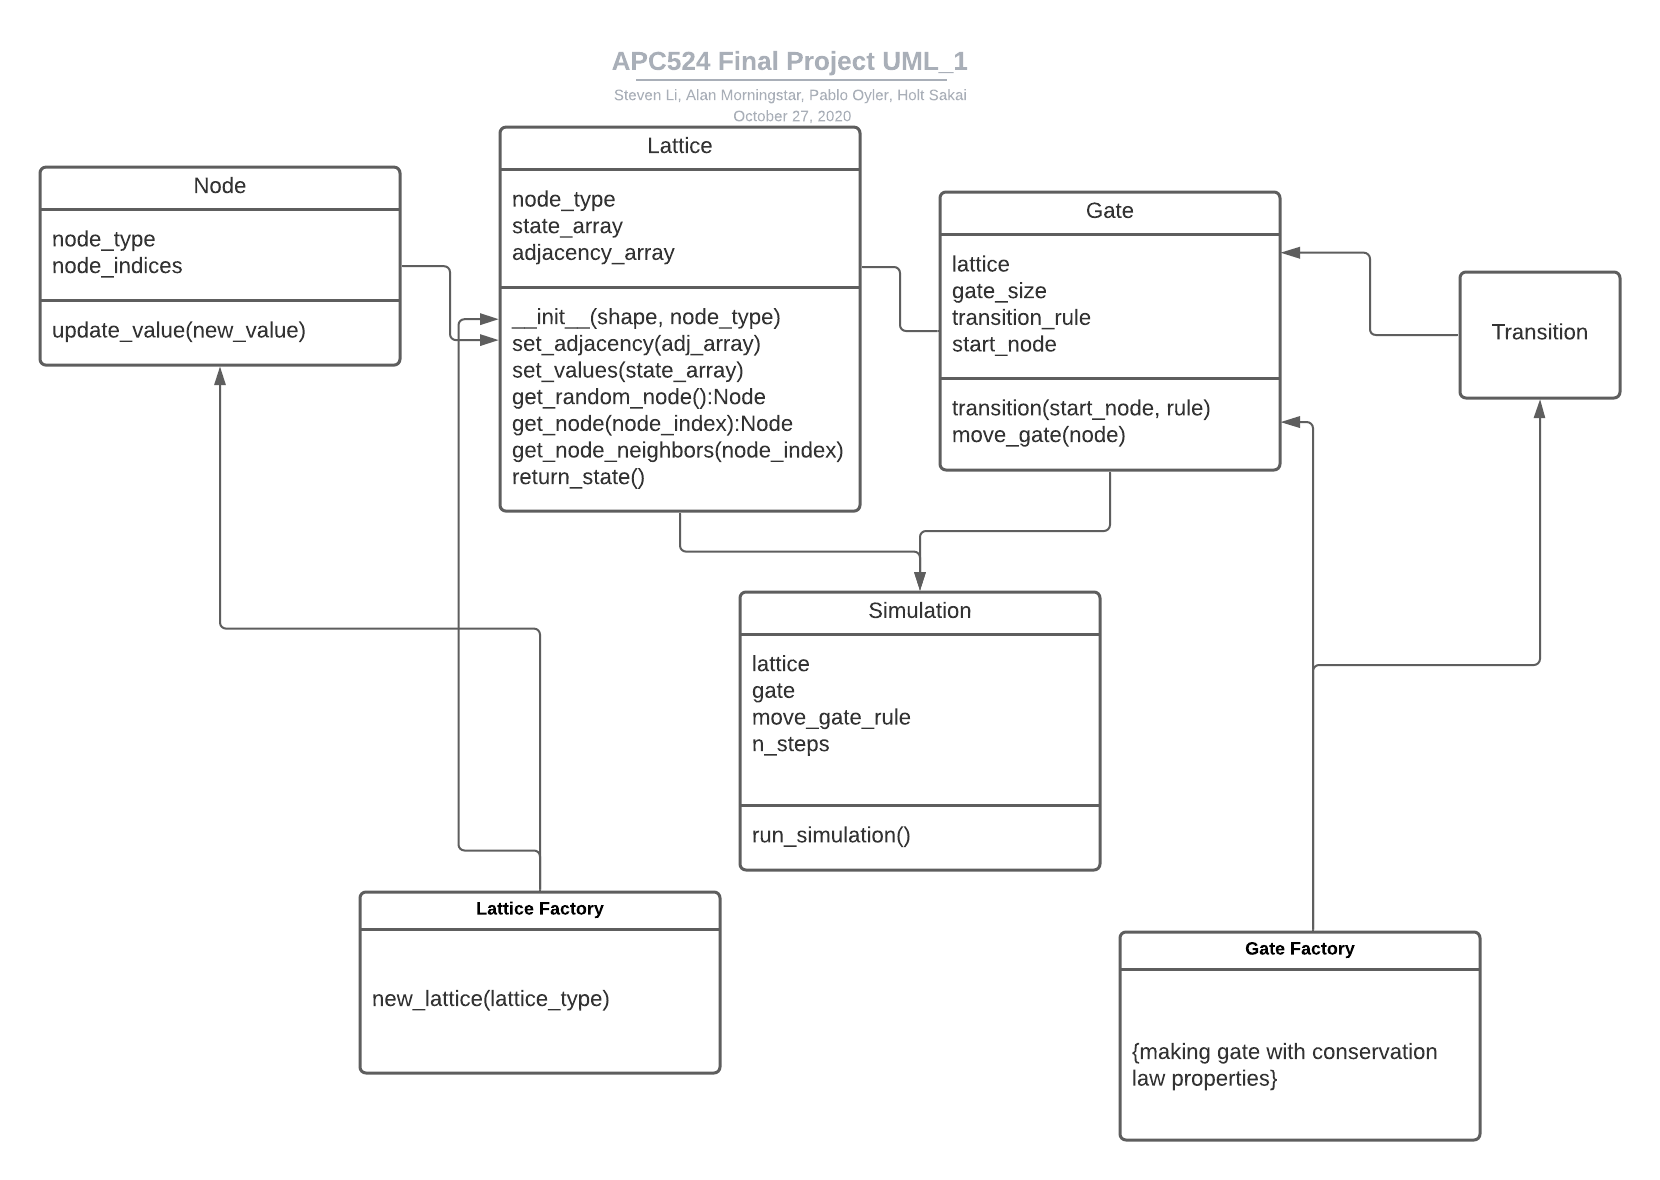
\includegraphics[width=1\textwidth]{APC524_FinalProject_UML.png}
    \caption{An early draft of the UML diagram which shows the high-level structure that we have followed thoughout the development process}
    \label{fig:uml}
\end{figure}

\subsection{Degree of freedom ($\texttt{apclattice.dof}$)}
In the $\texttt{dof}$ module we have implemented two common (in statistical physics models) types of degrees of freedom for lattice sites: discrete and continuous contiguous degrees of freedom. They are implemented as concrete subclasses of the abstract base class $\texttt{DOF}$. The $\texttt{DiscreteDOF}$ class takes on integers $\in [i_\mathrm{min}, i_\mathrm{max}]$, which is useful in, for example, the description of systems where the number of particles on a site is bounded. We also implemented a $\texttt{ContinuousDOF}$ class that takes on real values $\in [r_\mathrm{min}, r_\mathrm{max}]$. This could be useful in describing, for example, the ``XY"" model, where there is an angle $\theta_i \in [0, 2 \pi]$ of an arrow on each site $i$ of a two-dimensional (2D) lattice.

\subsection{Unit cell ($\texttt{apclattice.unitcell}$)}
In the $\texttt{unitcell}$ module we've implemented the class $\texttt{UnitCell}$, representing the basic repeating unit of a lattice, and subclasses $\texttt{HoneycombUnitCell}$, $\texttt{SquareUnitCell}$, and $\texttt{LineUnitCell}$. The latter three represent the unit cells with which the standard versions of the 2D honeycomb lattice, 2D square lattice, or 1D square lattice can be built. A unit cell is specified by a set of ``lattice vectors" $\vec{a}_i$, for $i\in [0, D-1]$ where $D$ is the spatial dimension, and a set of ``basis vectors" $\vec{b}_i$, for $i \in [0, S-1]$ where $S$ is the number of sites per unit cell. Lattice vectors are the translation vectors for building up the lattice using unit cell ``tiles", and basis vectors are the locations of sites within a unit cell. These sets of vectors are stored as lists of $\texttt{numpy.array}$ objects within the $\texttt{UnitCell}$. A $\texttt{UnitCell}$ also stores a list of $\texttt{DOF}$ objects that specify the degrees of freedom on each lattice site within the unit cell.  For example, a honeycomb lattice of sites can be broken up into repeating diamond-shaped unit cells with two distinct types of sites (see Fig.~\ref{fig:honeycomb}).

\begin{figure}[ht]
    \centering
    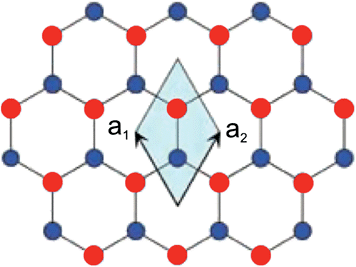
\includegraphics[width=0.5\textwidth]{honeycomb.png}
    \caption{Honeycomb lattice. Vectors $\mathbf{a}_1$ and $\mathbf{a}_2$ specify the discrete transnational symmetry of the honeycomb lattice. There are two distinct sites (red and blue) per unit cell (shaded light blue).}
    \label{fig:honeycomb}
\end{figure}

\subsection{Lattice ($\texttt{apclattice.lattice}$)}
In the $\texttt{lattice}$ module we provide the $\texttt{Lattice}$ class. This object contains a $\texttt{UnitCell}$ and information on how many times that unit cell is translated in each spatial direction to make up the lattice. It also has the option of periodic or open boundaries, and it stores the state that each site's degree of freedom is in, which gets updated when the lattice is ``time evolved". Much of the functionality of the $\texttt{Lattice}$ is to be able to conveniently query the data describing the lattice, such as the absolute position of each site of the lattice, or the map between the $\texttt{ind}$ of a site (an integer index $\in [0, n_s-1]$ where $n_s$ is the total number of sites in the lattice) and the $\texttt{coords}$ of a site (a tuple giving the Cartesian coordinates of the particular unit cell in the lattice that the site lives in and which site in that unit cell is the one). This is an $O(n_s)$ amount of data, so it is generated when a $\texttt{Lattice}$ is initialized and stored for lookup, instead of calculating it ``on the fly" as needed.

\subsection{Gate ($\texttt{apclattice.gate}$)}
In the $\texttt{gate}$ module we introduce the $\texttt{Gate}$ abstract base class and subclass it with the example of the $\texttt{HoneycombGate}$ class, which enacts charge-conserving dynamics on lattices that are built up from the $\texttt{HoneycombUnitCell}$ with discrete degrees of freedom. (Think of some fixed number of particles on a lattice, and the particles hop around locally. See demo at $\texttt{examples/demo.ipynb}$.) The way you apply a $\texttt{Gate}$ to a $\texttt{Lattice}$ is via the call ``dunder" method. If you have a $\texttt{Gate}$ $\texttt{g}$ and a $\texttt{Lattice}$ $\texttt{lat}$, then calling $\texttt{g(lat, i)}$ will apply the gate to the lattice at site $\texttt{i}$ (and whatever nearby sites are involved in the gate).

\section{Demonstration}
\label{sec:demo}
We provide a demonstration notebook in the examples directory. In the demo we set up a honeycomb lattice in which $0$ or $1$ particle can exist on each site. We first set up the empty lattice (no particles) and plot the structure of the lattice to visualize it (Fig.~\ref{fig:output}). We then go on to fill half of the sites that are closest to the central site, and we run the dynamics, applying charge-conserving gates at random locations in the lattice. Plotting throughout the time evolution allows us to see the initial blob of charge diffuse into the rest of the system, and at long times the system approaches an equilibrium where we can no longer tell where the initial blob of charge was placed. Please see $\texttt{examples/demo.ipynb}$.
\begin{figure}
     \centering
     \begin{subfigure}[b]{0.3\textwidth}
         \centering
         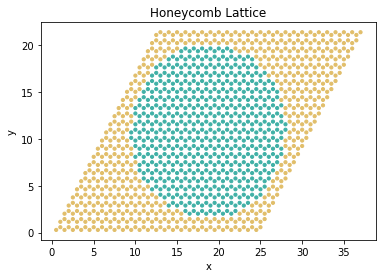
\includegraphics[width=\textwidth]{step0.png}
         \caption{Initial condition}
         \label{fig:s0}
     \end{subfigure}
     \hfill
     \begin{subfigure}[b]{0.3\textwidth}
         \centering
         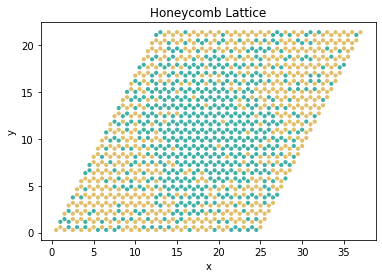
\includegraphics[width=\textwidth]{step8.png}
         \caption{8 time steps}
         \label{fig:s8}
     \end{subfigure}
     \hfill
     \begin{subfigure}[b]{0.3\textwidth}
         \centering
         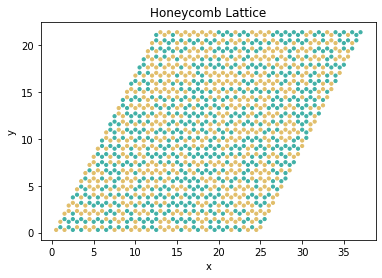
\includegraphics[width=\textwidth]{step32.png}
         \caption{32 time steps}
         \label{fig:s32}
     \end{subfigure}
        \caption{Output of the simulation after after various time steps}
        \label{fig:output}
\end{figure}

\section{Development process}
To develop this project we, at first, worked on separate submodules of the code so that little coordination was needed. We designed rough ideas of interfaces, and made suggestions to each other for modifications as we worked on our own submodules. We used git and GitHub pull requests to push chunks of completed code to a development branch of the project. After a skeleton of the code was completed, we found that it was often useful to block of periods of time where only one of us would review and edit the entire code, and make a pull request to incorporate those changes.

We found that testing was easier to keep up with for the simpler pieces of code like the $\texttt{dof}$ module. Once we got into the more complex submodules like $\texttt{gate}$ that interact with and rely on the other submodules, unit testing became a bit more challenging, because we were unsure if we should be breaking down the tests into proper atomic pieces.

\subsection{Workflow}
Near the beginning of the project, a significant amount of time was spent on choosing and learning a git workflow.  The one we chose can be best described by Fig.~\ref{fig:wf} below.  
\begin{figure}[ht]
    \centering
    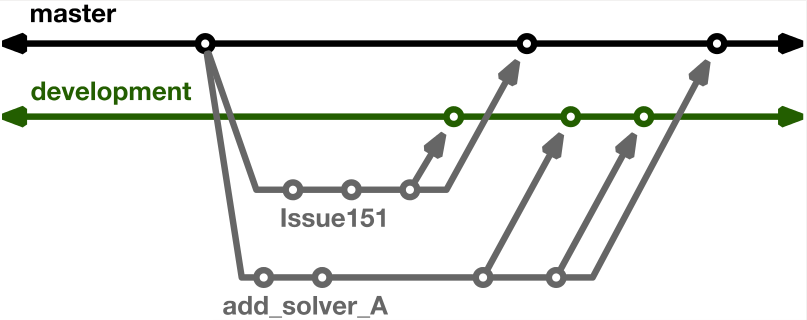
\includegraphics[width=0.8\textwidth]{index.png}
    \caption{Our workflow is very similar to this workflow diagram by David Bernholdt as presented in class.}
    \label{fig:wf}
\end{figure}

Each user works on their own branch.  At any given time the team decides on who will be working on which file so that no two people are working on the same file at the same time.  There is a development branch named $\texttt{dev}$ that they send pull requests to but individually, they each work on their own branch with commits until they have completed the task they want to do for the file they are working on.  From that point, the instruction is as followings:

\begin{enumerate}
    \item From their feature branch, run $\texttt{git push origin their\_feature}$.
    \item Run $\texttt{git checkout dev}$.
    \item Run $\texttt{git pull}$ with their credentials.
    \item Go to GitHub and deal with the pull request. (See Sec.~\ref{sec:pr}.)
    \item Run $\texttt{git checkout their\_feature}$.
    \item Run $\texttt{git merge dev}$ to synchronize the two branches.
    \item Continue working on $\texttt{their\_feature}$ or create a new one.
\end{enumerate}

\subsubsection{Pull request}
\label{sec:pr}
After the pull request is made on the individual computer, one of the team members (which has soon devolved to oneself) manages the pull request on GitHub.  GitHub checks for merge conflict (later then augmented by Travis CI for running tests, as described in Sec.~\ref{sec:ci}) and if all goes well, the pull request will be confirmed then merged to $\texttt{dev}$.  On the local machine, $\texttt{dev}$ is pulled then merged to the individual member's feature branch.  Luckily, no merge conflict was encountered during the entire process due to the small number of team members and deciding from the beginning that no two people will be working on the same file at the same time.

\subsubsection{Major revisions}
There were three major revisions to the high-level structuring of the code.  The first was organizing files into a more organized folder structure.  This was completed live with everyone on Zoom so that everyone was able to get their branches onto $\texttt{dev}$.  The second major revision was the migration of the entire GitHub repository from Holt's account to Alan's account.  This process involved the finalization of the files created by Holt (then later Pablo) to make sure compatibility is still maintained.  Some restructuring of how classes are distributed between files are made.  Lastly, classes were combined to fewer files to improve the readability of the structure, which, in retrospect, have deviated from the intentions of the course to create a sustainable package that is amenable to future development.

\subsubsection{Workload}
As the originator of the project idea, Alan served as the project lead that directed the goals and aspirations for the project.  Alan managed the Git repo and created most of the high-level aspects of the code.  Steven was responsible for the specific instantiations of $\texttt{UnitCell}$ (as well as a $\texttt{UnitCellFactory}$ class that was never implemented in the demo).  Steven was also responsible for some of the managerial aspects of the projects including organizing meetings and communication.  Before dropping the class, Holt served as the repo manager as was responsible for the $\texttt{Lattice}$ and $\texttt{UnitCell}$ classes and Pablo create the $\texttt{\_\_init\_\_.py}$ files for package management as well as a major contributor of the project proposal.  Despite the various adversities encountered throughout the project, the team managed to pull it together to produce a functioning lattice simulator.

\subsection{Continuous integration}
\label{sec:ci}
Continuous integration (CI) was done using the Travis framework. Our test suite is run each time we commit to the repository.  Both the built and unit tests are completed within seconds and did not significant lengthen the workflow process.  This is partly due to the fact that all of the tests run are unit tests, which only checks for the integrity of the individual classes.  We imagine that a high level test (for example, the whole simulation) would take much longer as the simulations take much longer to run, which leads us to the next section.

\subsection{Profiling}
The profiling process was completed on the demo (Sec.~\ref{sec:demo}). We used the IPython magic commands $\texttt{\%timeit}$ and $\texttt{\%prun}$. We found that when running the simulated dynamics in the demo, the average time it took per gate application was about $200\ \mu$s. By examining the output of $\texttt{\%prun}$ we can see that what takes the most time in the dynamics are the calls to $\texttt{numpy.random.randint}$ which is used to sample new states for the sites of the lattice.  This command was improved from a previous call $\texttt{numpy.random.choice}$ which had a 20\% longer run time.  An attempt was made to use $\texttt{\%lprun}$ and $\texttt{\%mprun}$ using the $\texttt{line\_profiler}$ and $\texttt{memory\_profiler}$ packages, respectively, but we were unable to get it to produce a desirable output.

\subsection{Documentation}
Documentation was generated using Sphinx's autodoc feature. We followed the reStructured text format for our docstrings, which allowed for full automatic documentation. Instructions for building the docs are in the README of the project repository.

\section{Outlook}
At this point the code is not performance, so it could use some effort in optimization. We could also build a simulation module that allows a user to more easily run simulations. A starting point for a simultion module is the code in our demonstration. Testing is also somewhat incomplete. It could be broken down more atomistically, and the tests are not well-explained or documented at the moment.  High level tests that checks for the correctness of the simulation results could also be implemented by comparing with other packages or analytical results.

\section{Acknowledgements}
The authors would like to thank Holt Sakai and Pablo Oyler for their early contributions to the project and ensuring a smooth transition despite deciding to drop the class.  We like to thank Gabe and the AIs---Yixiao and Dev---for accommodating our extenuating circumstances.  We would also like to especially thank Gabe for providing this class and the informative overview and practice of the various aspects of the software development process.

\end{document}
